%!TEX root = ../../../thesis.tex

\chapter{Guide to Using NEFI}\label{app:nefi}

	Here we document our experiences with using \NEFI. As discussed in \Fref{chap:nefi}, the combination of input image quality and \NEFIs segmentation algorithms makes or breaks the resulting graph. Let us first discuss the properties of ideal and non-ideal input images. Our goal is to give the prospective user an idea of what to avoid and what to look out for regarding inputs. Furthermore, we add some pointers on how to deal with challenging inputs and what one can try to do in order to improve the output of \NEFI. 

\section{Properties of Ideal and Non-ideal Images}

	Since, the determining factor of the quality of \NEFIs graph extraction is the segmentation step, ideal images should enable a nearly perfect separation of foreground and background. Such images should have a high contrast between the depicted structures of interest and the background. At the same time it is very important that images are free of strong reflections or shadows because such areas are likely to show an even higher contrast to the background than the actual structures of interest. As a result, the segmentation algorithms are prone to identify these regions as foreground causing the actual structures of interest to be ignored. The presence of strong color or brightness gradients can have similar detrimental effects and should thus be prevented if possible. See \Fref{fig:sup:reflection} and \Fref{fig:sup:gradient} for examples of challenging images which \NEFI will have difficulties working with.

	\begin{figure}
		\centering
		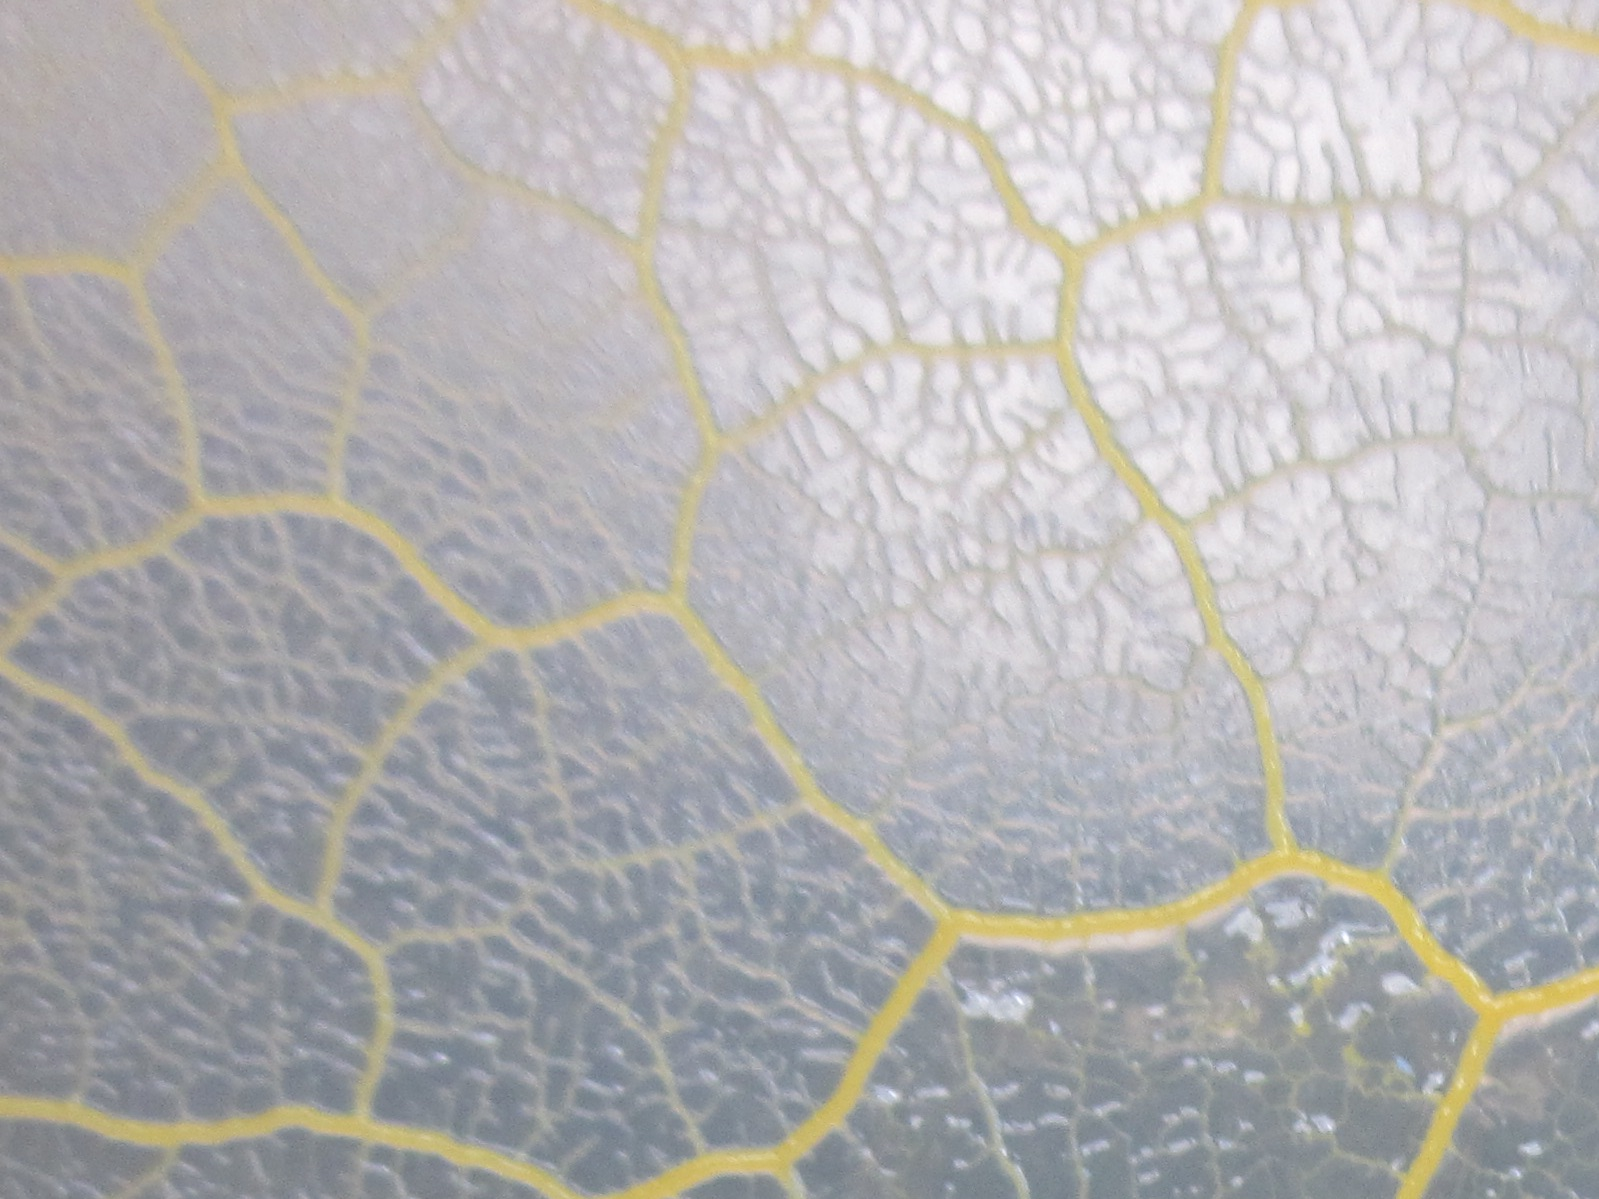
\includegraphics[width=0.5\linewidth]{reflections.jpeg}
		\caption[\NEFIs caveats - Reflections]{This image of \P contains strong light reflections in the upper right quadrant which will cause \NEFIs segmentation algorithms to be lead astray. The fact that the image is not properly focused is less of a problem in comparison.}
		\label{fig:sup:reflection}
	\end{figure}

	\begin{figure}
		\centering
		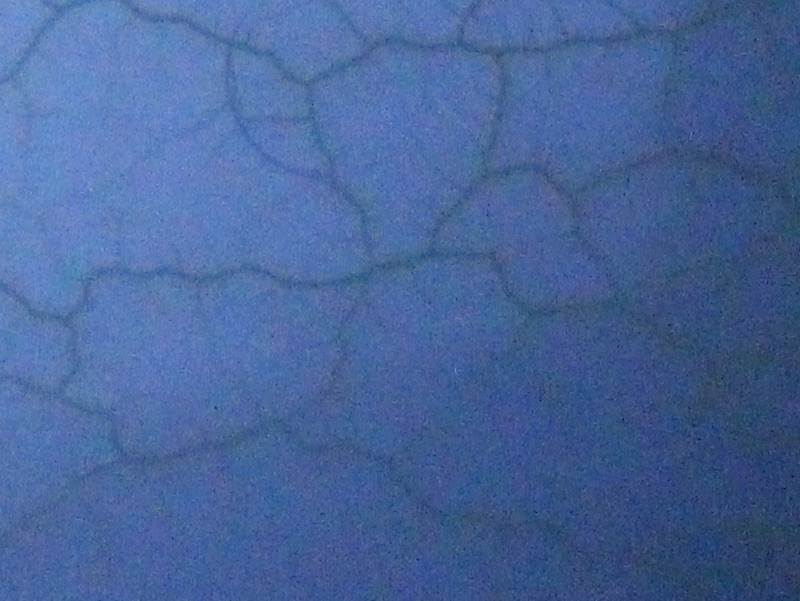
\includegraphics[width=0.5\linewidth]{gradient.jpeg}
		\caption[\NEFIs caveats - Gradients]{This image of \P was not illuminated evenly from below. As a result it contains a brightness gradient which is detrimental for many of the segmentation algorithms currently implemented in \NEFI. The fact that the image contains a lot of visible noise makes it a bad candidate for processing with \NEFI.}
		\label{fig:sup:gradient}
	\end{figure}

	Another factor that influences segmentation, and by extension graph detection, are contaminations of different origin. Examples include parts of the image which might not belong to the object of interest at all. Such regions should be removed before loading the image into \NEFI, see \Fref{fig:sup:petri_dish}. 

	\begin{figure}
		\centering
		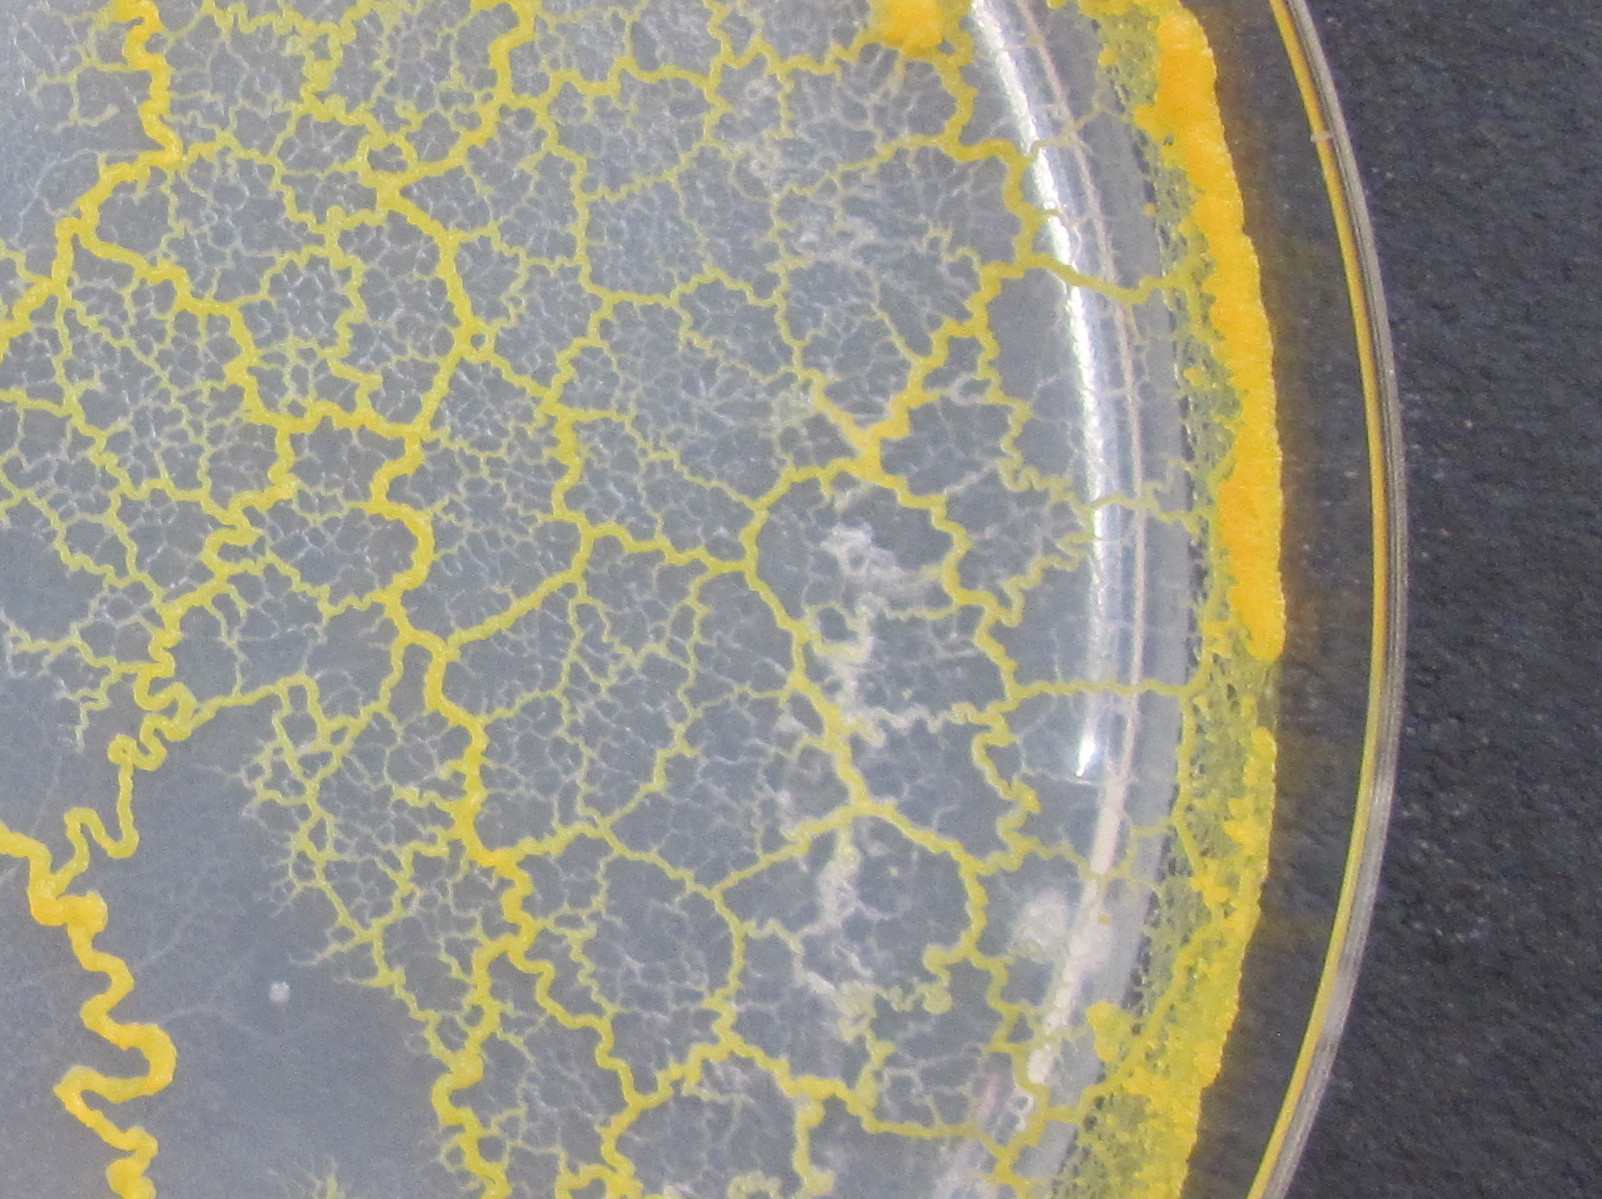
\includegraphics[width=0.5\linewidth]{petri_dish.jpeg}
		\caption[\NEFIs caveats - Non-network objects]{In addition to the network of \P the image contains the edge of a petri dish and pieces of the background on the right hand side (as well as light reflections). Prior to any attempt of processing the image, petri dish and background should be removed.}
		\label{fig:sup:petri_dish}
	\end{figure}

	\Fref{fig:sup:clutter} depicts an image lacking in a similar way. The image contains objects that are technically part of the network one would be interested to extract, however, they are not suited very well to be represented as a graph. In particular, they will be picked up correctly in the segmentation step yielding four large areas of white pixels. Subsequently, thinning will try to reduce these to lines resulting in more or less unpredictable results. While the remaining parts of the structure will be processed correctly, such images do not constitute ideal candidates for processing with \NEFI.

	\begin{figure}
		\centering
		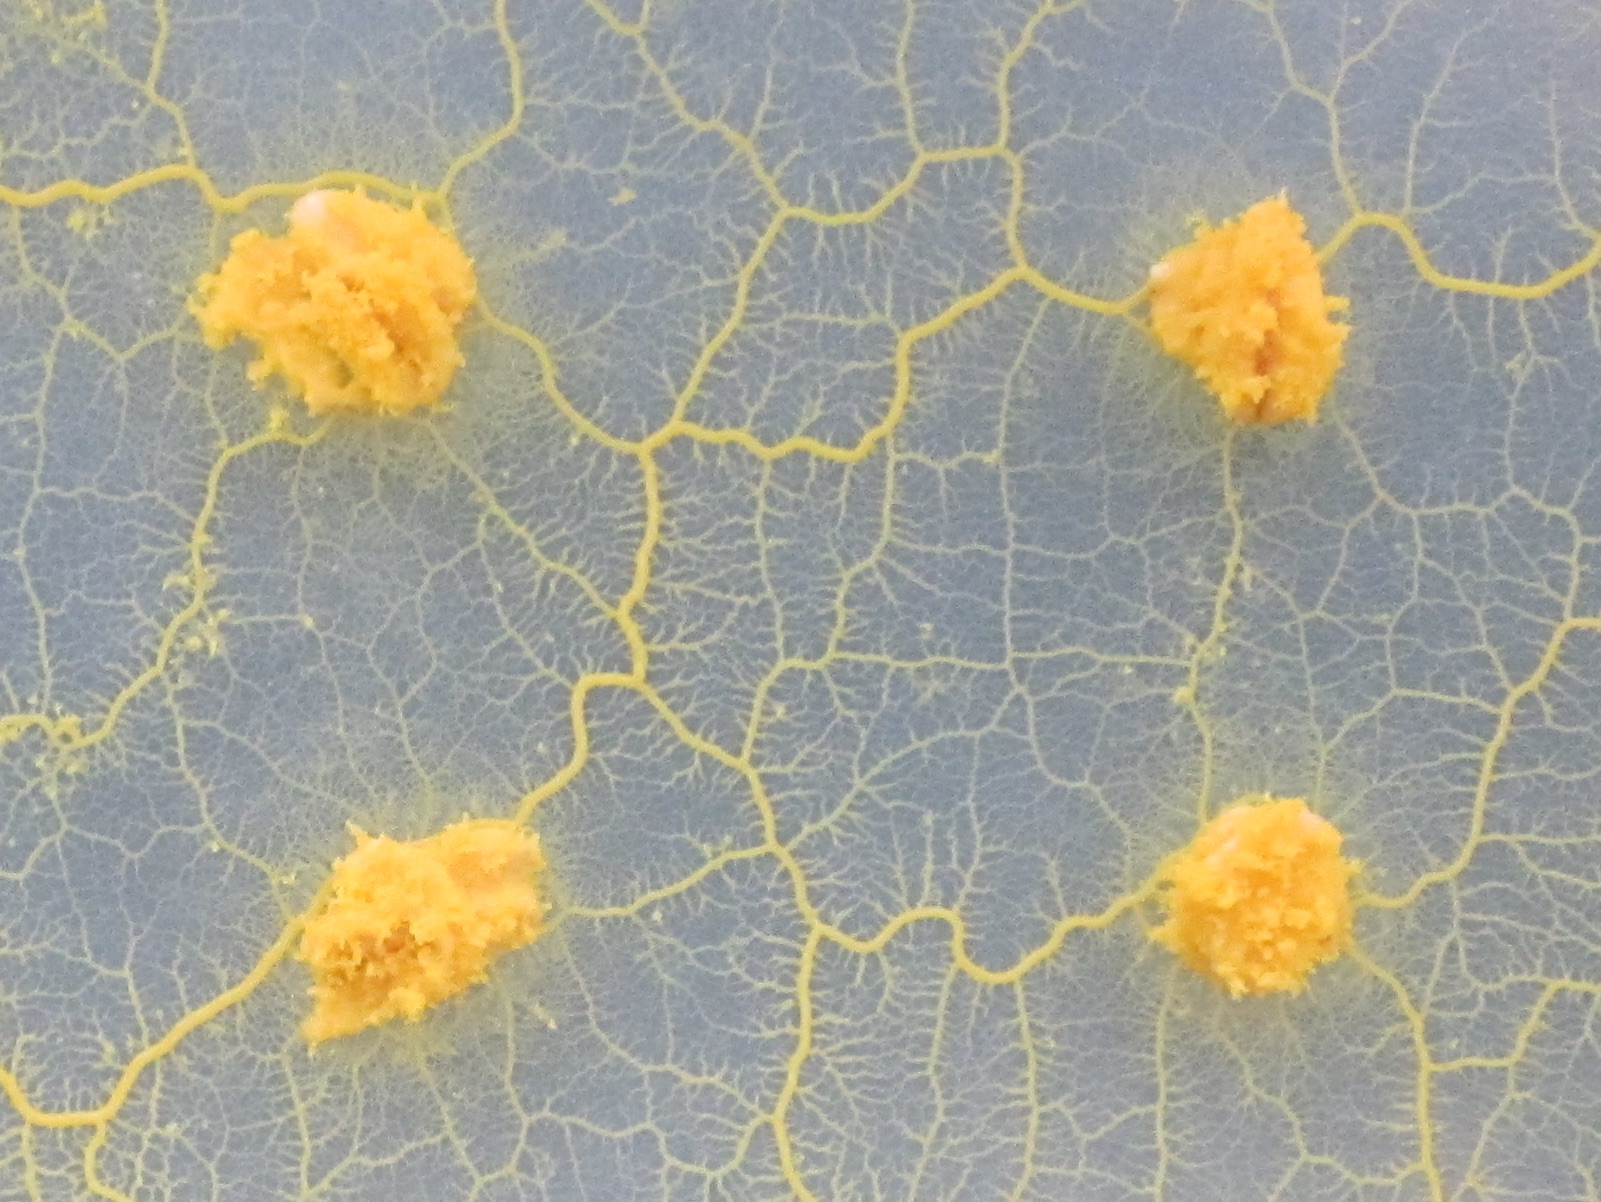
\includegraphics[width=0.5\linewidth]{clutter.jpeg}
		\caption[\NEFIs caveats - Non-network objects]{The network of \P depicted in the image contains 4 massive, non-network-like regions (oat flakes completely covered by the mold). After segmentation, thinning will try to reduce these regions to lines leading to unpredictable results. The remaining parts of the network, however, will be extracted correctly.}
		\label{fig:sup:clutter}
	\end{figure}

	\newpage

	Summarizing this information we have the following desirable properties for an ideal image:

	\begin{itemize}
		\item High contrast between foreground and background.
		\item Uniform background void of reflections, shadows as well as color or brightness gradients.
		\item No contaminations that might disrupt the segmentation process.
	\end{itemize}

	When producing images to be processed with \NEFI one should strive to fulfill these properties whenever possible. See \Fref{fig:sup:good1} and \Fref{fig:sup:good2} for examples of very good input images.

	\begin{figure}
		\centering
		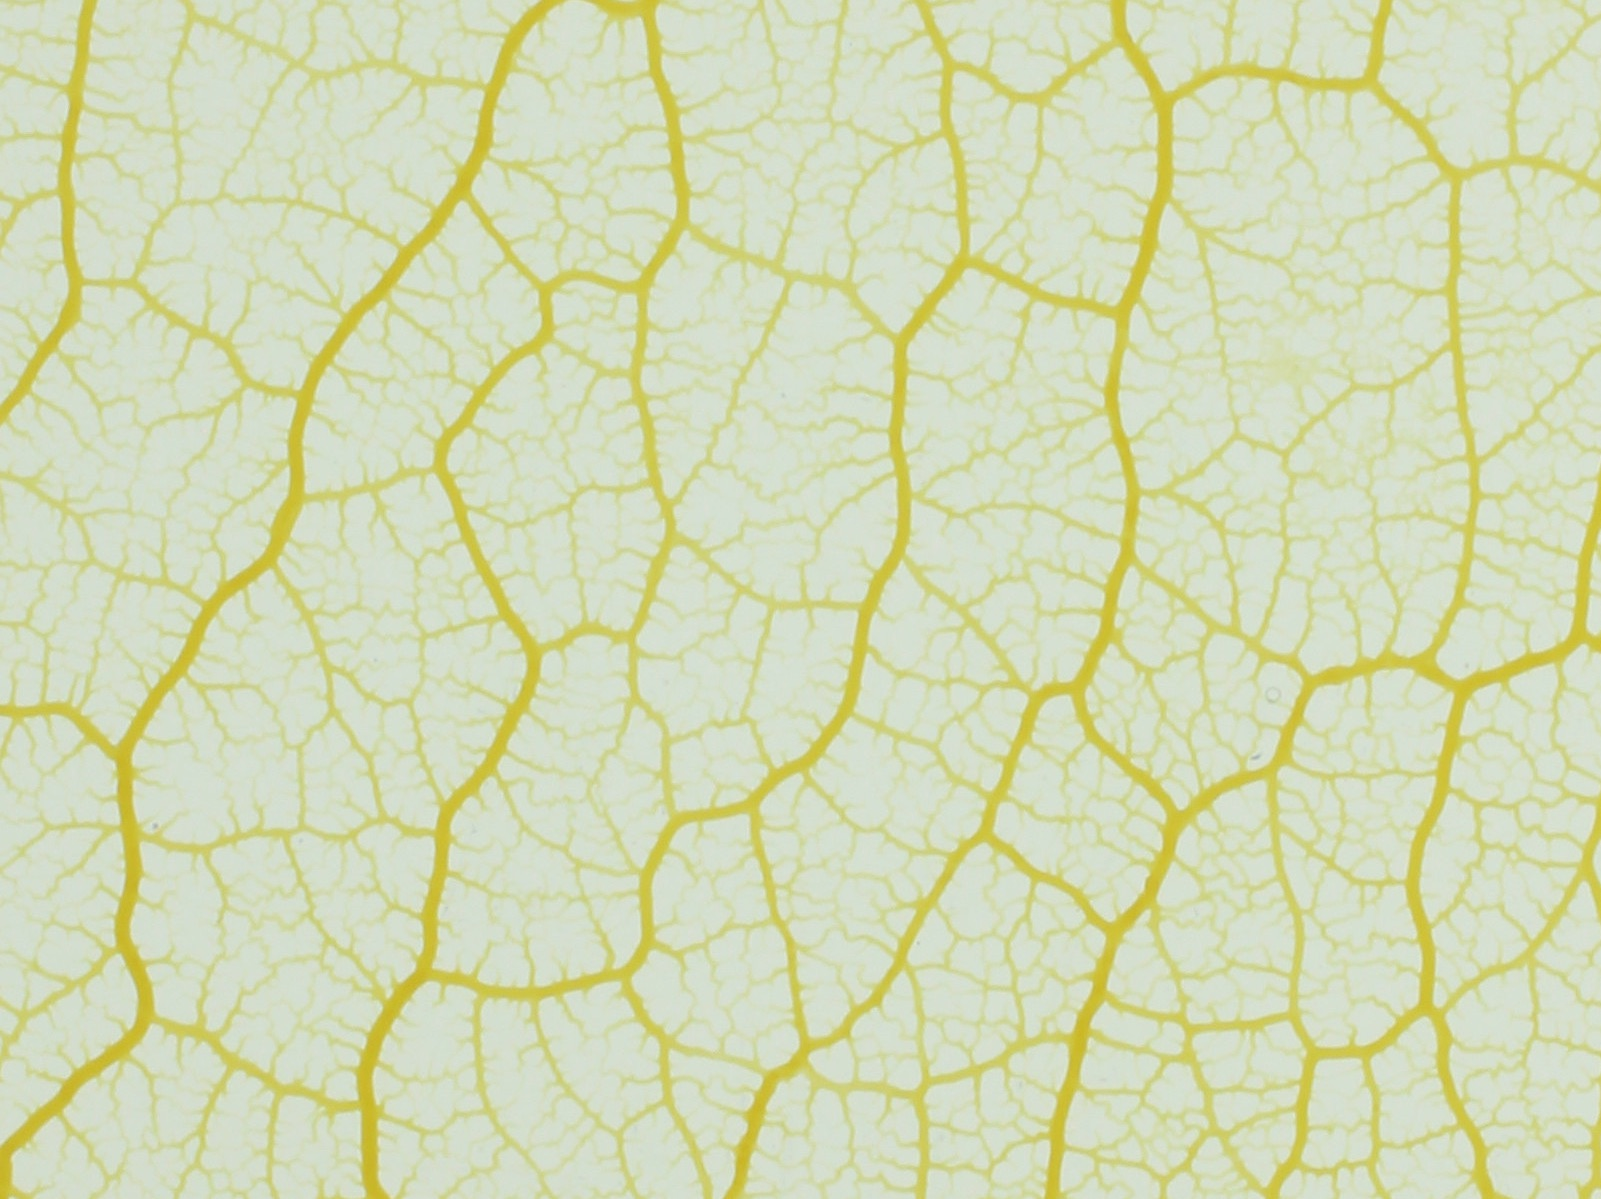
\includegraphics[width=0.5\linewidth]{perfect_physarum.jpeg}
		\caption[\NEFIs strengths - An ideal image of \P]{An ideal image of \P. The image has been obtained using bright field illumination and was produced in a collaboration with the KIST Europe.}
		\label{fig:sup:good1}
	\end{figure}

	\begin{figure}
		\centering
		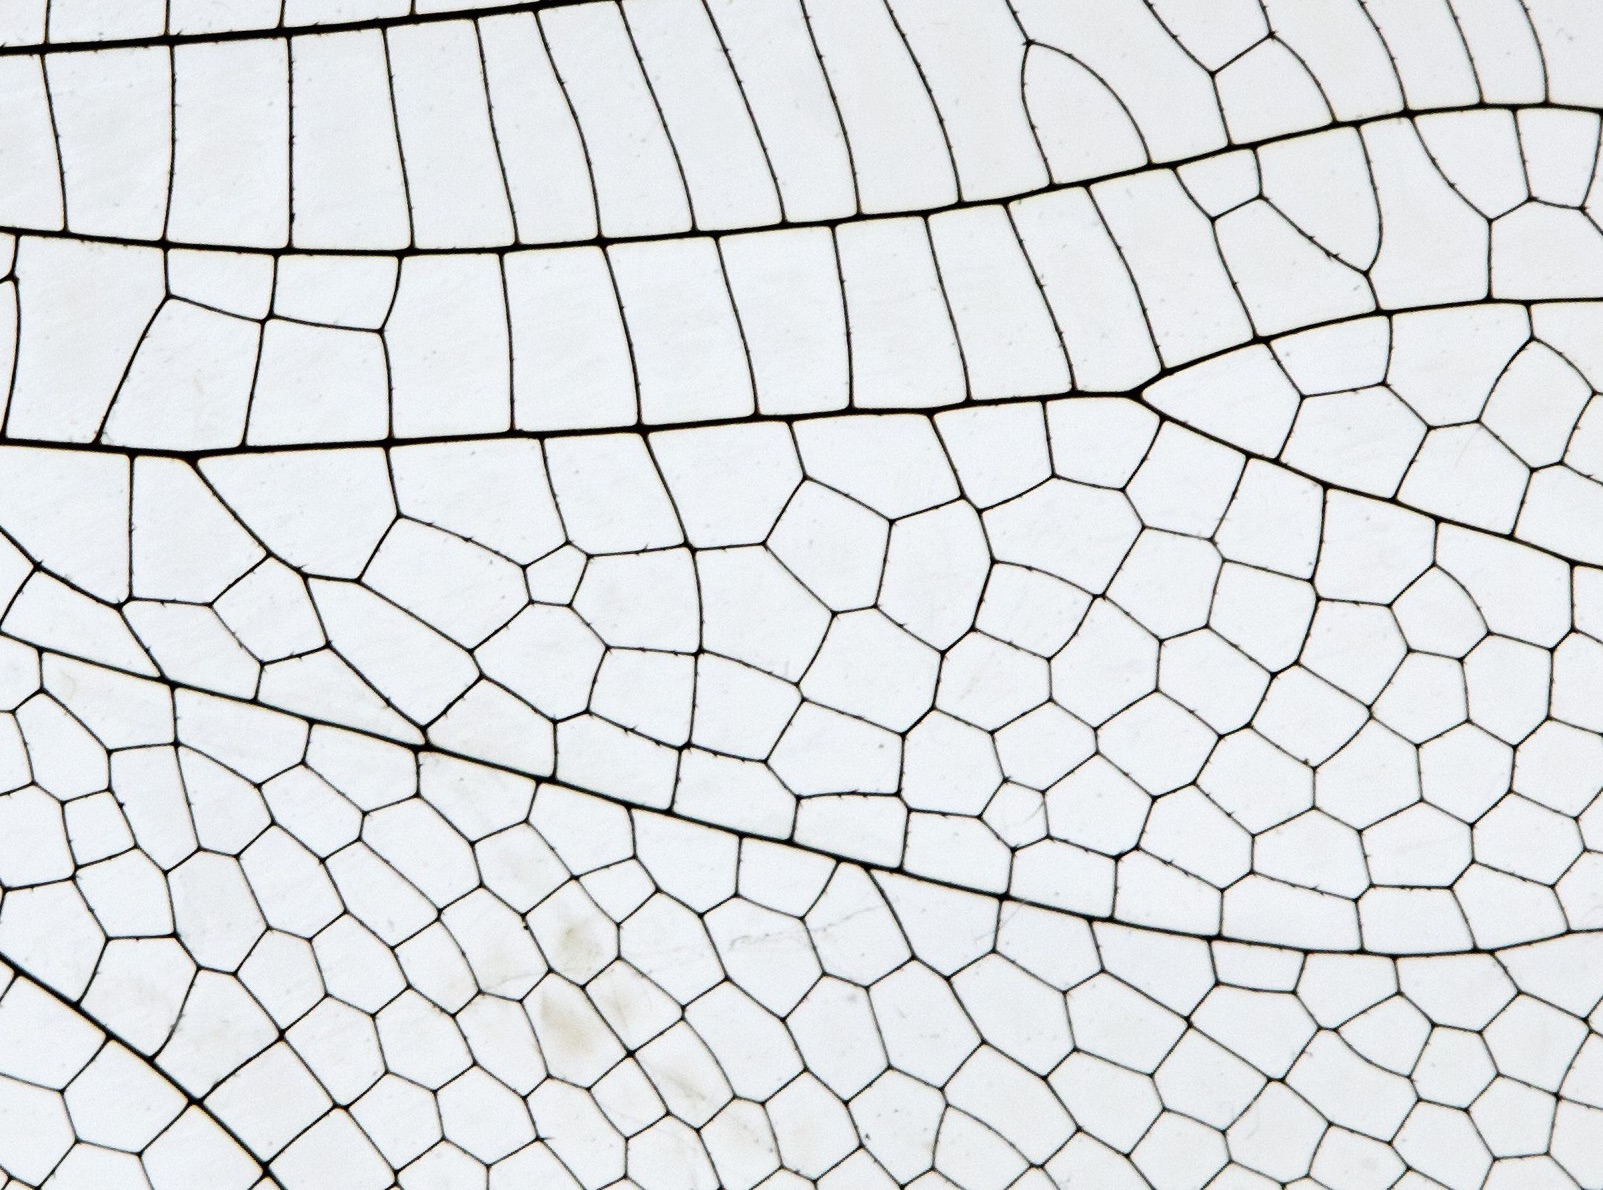
\includegraphics[width=0.5\linewidth]{perfect_dragonfly.jpeg}
		\caption[\NEFIs strengths - An ideal image of \A]{An ideal image depicting a detail of the wing of \A. Image courtesy of Pam and Richard Winegar.}
		\label{fig:sup:good2}
	\end{figure}
 
\section{Dealing With Challenging Images}

	\NEFI operates best on images produced under controlled laboratory conditions that fulfill the properties described in the last section. However, more difficult inputs may still be processed, but most likely at the cost of reduced quality. Based on our experience when dealing with more challenging input and the results of our evaluation, we are able to formulate the following recommendations for the usage of \NEFI:

	\begin{description}
	\item [Otsu's method] may be used on noisy or blurred images. It will do reasonably well as long as the image has a high contrast between network and background. Adaptive threshold, watershed based on adaptive threshold, and GrabCut with deletion and erosion may even perform slightly better under these conditions. Otsu's has the advantage that no parameters have to be set in order to get good results. The choice should be based on the desired degree of resolution of the extracted graph. We would recommend these methods to process \Fref{fig:sup:petri_dish} after removing areas that are not of interest.

	\item [Adaptive threshold and watershed based on adaptive threshold] may\\be used if differences in contrast between foreground and background are local and not too strong. If this is the case, good results may still be obtained. Both methods allow to analyze images that contain a color gradient in the background or that contain edges which have differing levels in brightness. One might try to process images like \Fref{fig:sup:reflection} and \Fref{fig:sup:gradient} with these methods while experimenting with different parameter settings. However, such images remain challenging. \NEFIs current algorithms may not deliver sufficient results.

	\item [Preprocessing methods] like Gaussian and Median Blurring, Denoising as well as Bilateral Filtering can be used to remove small artifacts, contaminations or irregularities from the image. Although these methods can reduce the amount of artifacts produced during segmentation and thinning, improvements come at a price. For example, imposing a strong blur causes the depicted edges to appear slightly wider. This effect will propagate through the pipeline causing the edge widths of the final graph to overestimate the true widths depicted in the image. We recommend to use preprocessing with care especially if a high accuracy regarding edge weights is required.

	\item[Graph filtering] enables the removal of unwanted artifacts and spurious vertices caused by irregularities in the input which propagate through the pipeline. However, filtering can only repair the result up to a given point. While the ability to add custom filters is powerful, it appears pointless to filter a graph established on the basis of a failed segmentation. We encourage users to visually verify the integrity of the established graph and only then to proceed with filtering.
	\end{description}

	We anticipate users to encounter images \NEFIs algorithms will be unable to handle properly. In this situation the user will have to rely on different segmentation solutions. 

	As a first suggestion, we recommend to user to look for available software specializing in segmentation. In this regard we like to point out the Kitware,~\href{http://www.itk.org/itkindex.html}{ITK Project}~\cite{ITKSoftwareGuideThirdEdition}. It's \emph{C++} code base has been developed by the medical image processing community and serves as the basis for many other specialized tools that deal with image processing as well as segmentation. 

	After a segmented image has been obtain using specialized third party segmentation software, \NEFI can take this image and proceed with graph detection and filtering directly.

	If no proper software is available, the user has the option to extend \NEFIs segmentation capabilities by adding more sophisticated code. When doing so, one can built on top of existing features already implemented in \NEFI. The literature offers a wealth of different approaches to segmentation leading to algorithms of varying complexity. Before diving into any implementation efforts, we strongly recommend to survey existing methods and their domains of effectiveness by consulting~\cite{chellappa,Pal19931277,pham2000current}.
